% !TeX root = ../mde-presentation.tex

\section{Implementation} \label{sec:implementation}

\subsection*{Core} \label{sec:core}

\begin{frame}{Core} \label{frm:core}

    \begin{columns}[T]
        \begin{column}{0.4\textwidth}
            \only<1>{
                The core package of the Model Data Explorer,
                \lstinline|mde-core|, implemented with Django, implements
                so-called \textit{Datasets}. A dataset might be identified
                with a specific experiment to run a model. It gets a unique
                handle and UUID and serves as a kind of namespace for the
                services associated with it. This makes resources related to a
                dataset better findeable as everything is linked to a specific
                dataset.
            }

            \only<2>{

                \lstinline|mde-core| additionally implements data groups.
                This can be anything from a project to a department or an
                institution. DataGroups can own datasets and they will be listed
                on their detail page. DataGroups can also own other DataGroups and
                as such inherit ownerships on the datasets.

                \lstinline|mde-core| uses a directed acyclic graph implementation
                \citep{OmenApps2021} to efficiently manage data group relations
                and permissions.
            }


        \end{column}
        \begin{column}{0.55\textwidth}
            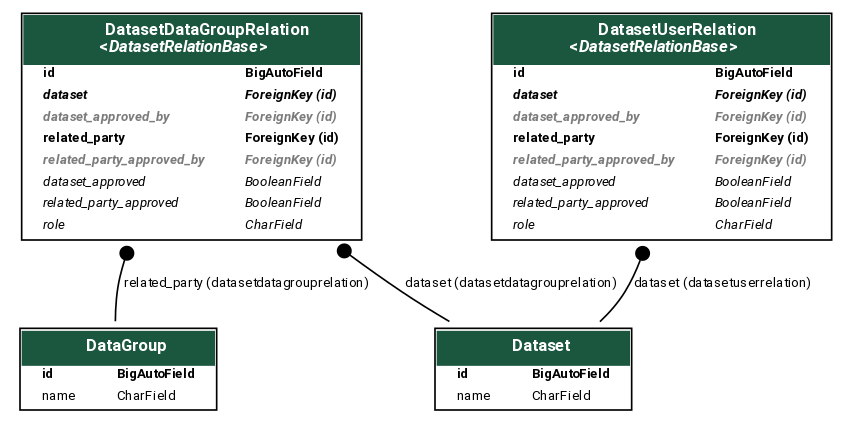
\includegraphics[width=\textwidth]{figures/dataset-datagroup.png}
            \only<2>{
                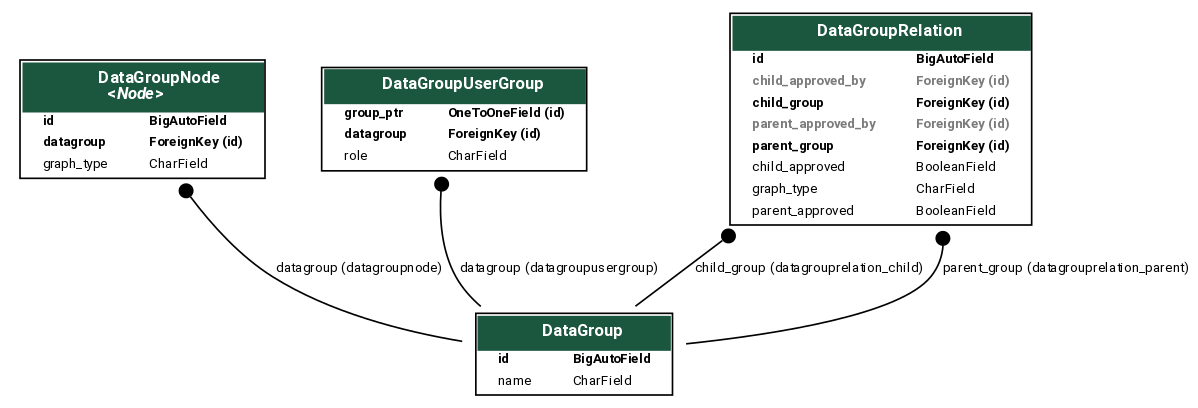
\includegraphics[width=\textwidth]{figures/datagroup-implementation.png}
            }
        \end{column}

    \end{columns}

    \begin{textblock*}{\textwidth}(0.05\linewidth, 1.07\textheight)
		\slidebuttons
	\end{textblock*}

\end{frame}

\begin{frame}{DataGroup relations}

    \label{frm:datagroup-relations}

    \begin{columns}[T]
        \begin{column}{0.4\textwidth}
            \begin{block}{In Research}
                \begin{itemize}
                    \item Many partners are involved in different projects
                    \item Data managers need to be able to configure metadata and create services
                    \item Relations should be built from the metadata and vice-versa
                \end{itemize}
            \end{block}
        \end{column}
        \begin{column}{0.55\textwidth}
            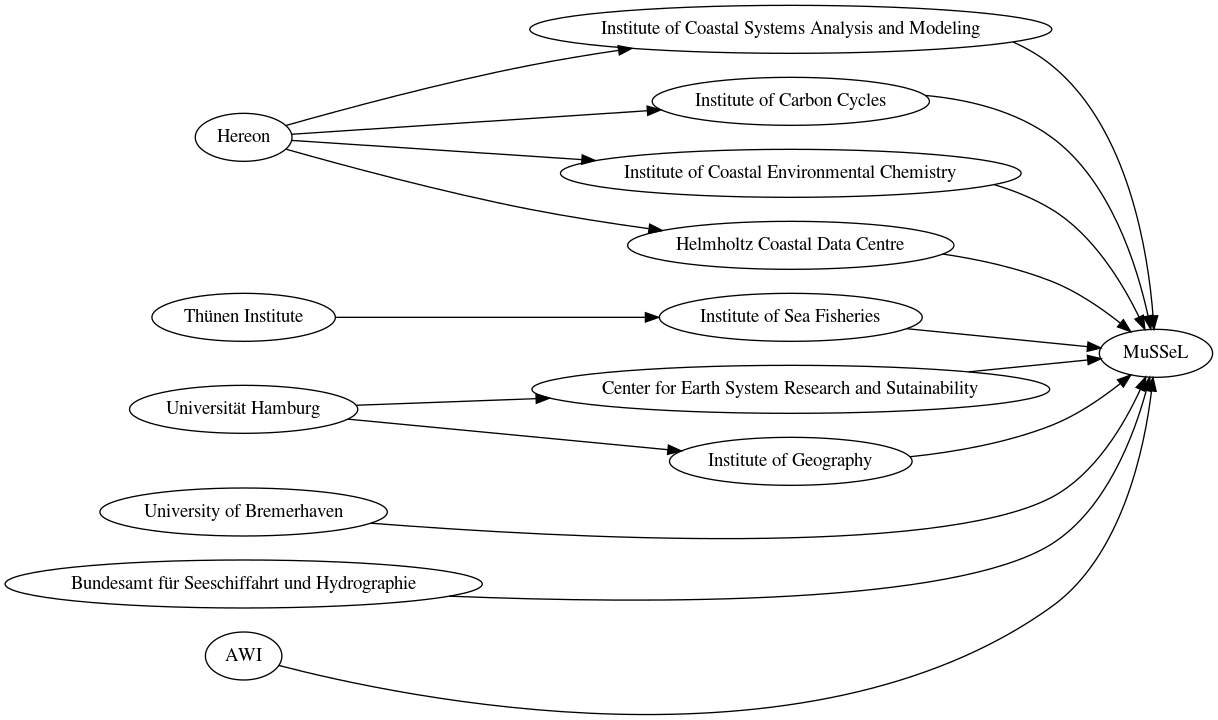
\includegraphics[width=\textwidth]{figures/datagroup-tree.png}
        \end{column}

    \end{columns}

    \begin{block}{In the Model Data Explorer}
        \vspace{0.5em}
        \begin{tabular}{p{0.5\textwidth}p{0.5\textwidth}}
            \tabitem Relationships between groups are
                \par \hspace{1.5ex} represented with a directed acyclic graph &
            \tabitem \indent Each institute, department, unit, project,
                \par \hspace{1.5ex} etc. gets its own page \\
            \tabitem Datasets are shown on each group site &
            \tabitem Maintainability is guaranteed through data
                \par \hspace{1.5ex} group relations
        \end{tabular}
    \end{block}

\end{frame}